\section{Siamese Multi-Object Tracking}
\label{sec:SiamMOT}

This section is dedicated to the most important tracker we have encountered during our research, called \siammot{}~\cite{shuai2021siammot}. Its importance stems from the fact that the majority of our experiments adopted this model. Even though this section could be part of the theoretical foundations chapter, we found it more comprehensible to provide the description of the base architecture closer to the description of our methods and experiments.

\subsection{General Description}

The authors of~\cite{shuai2021siammot} tracker focused on improving online \gls{mot}. As far as their methodology was concerned, they employed region-based approach~\cite{ren2017fasterrcnn} in conjunction with a Siamese multi-object tracking network, hence the name \siammot{}. Broadly speaking, this architecture employes Siamese tracker for motion estimation between two frames. We would like to note that all the principles so far discussed regarding Siamese trackers apply here. However, as already suggested, the adoption of \gls{rpn} enables this framework to have more information available. Not only there is the motion prediction from the Siamese tracker, there are also detections produced by the \modelname{Faster R-CNN} object detector~\cite{ren2017fasterrcnn} that is integrated within the whole architecture. Subsequently, an online solver is utilized to merge these prediction obtained from the tracker and detector heads. It is no surprise that such a framework that exploits modern approaches (more on that later) to object detection and Siamese tracking produces \gls{sota} performance.

We will disect this framewrok in great detail since we studied it scrupulously. We performed multiple experiments, many of which did not yield expected improvements. Nevertheless, the practical part of our work was focused on contributing to the open source repository dedicated to this project developed by several Amazon researchers~\cite{websiammotoriggithub}. We followed a standard path of how contributing to open source projects should be done in a transparent and, more importantly, compatible fashion. We initialized a fresh fork of this project on our personal GitHub account~\cite{websiammotforkgithub} to preserve as much compatibility with the original software as possible and to not strip ourselves of the opportunity to easily receive potential updates from the original repository.

During our development we often engaged in discussions related to this project incentivized by other researchers who were also working on this project and trying to either only apply this work to their specific use case or even extend the model. Our detailed knowledge of this model acquired through deliberate and long-lasting work on this project often helped several other programmers who dealt with various issues. From the programming standpoint, our work involved a considerable amount of programming, even though the base architecture was provided and fully functional. We would like to emphasize that the project consisted of $?$ lines of source code programmed purely in Python programming language. Concerning the deep learning aspect, the PyTorch library~\cite{paszke2019pytorch} was primarily used. It is a widely known library aimed at building deep neural network models while exploiting automatic differentiation.

\subsection{Model Architecture}

The two key aspects of the the \siammot{} architecture are \modelname{Faster R-CNN}~\cite{ren2017fasterrcnn} object detector and Siamese tracker. The salient element of the \modelname{Faster R-CNN} is the \gls{rpn}. Simply put, \siammot{} adds a region-based Siamese tracker along the standard $2$-stage object detection pipeline in order to model instance-level motion.

As depicted in Fig.~\ref{fig:SiamMOTArchitecture}, the input consists of two frames, namely $\mtxsup{I}{t}$ and $\mtxsup{I}{t + \delta}$, accompanied by a set of detected object instances $\mtxsup{R}{t} = \cbrackets{\subsup{R}{1}{t}, \subsup{R}{2}{t}, \dots, \subsup{R}{i}{t}, \dots}$ at time $t$. During the inference process, the detection head produces a set of detected object instances $\mtxsup{R}{t + \delta}$ whilst the tracker's task is to propage the detections $\mtxsup{R}{t}$ to time $t + \delta$, and thus yielding the tracker output denoted as $\mtxsup{\tilde{R}}{t + \delta}$. Please note that it is not the output of the entire tracker, only of the Siamese tracker itself. These instances have to be further processed. Explained next.

This framework relies on a motion model that \emph{tracks} each detected object instance from time $t$ to $t + \delta$. A specific \gls{bbox} $\subsup{R}{i}{t}$ at time $t$ is thus propagated to its future counterpart $\subsup{\tilde{R}}{i}{t + \delta}$ at time $t + \delta$. Such a procedure is then completed by a spatial matching process the objective of which is the \emph{association} of the tracker output $\subsup{\tilde{R}}{i}{t + \delta}$ with detections $\subsup{\tilde{R}}{i}{t + \delta}$ at time $t + \delta$ such that detected instances are linked from $t$ to $t + \delta$.

Assume there is a specific object instance $i$ detected at time $t$. Then, the Siamese tracker searches for this particular instance at frame $\mtxsup{I}{t + \delta}$ while exploiting a contextual window spanning a fixed neighborhood of the object's location (i.e., $\subsup{R}{i}{t}$) at frame $\mtxsup{I}{t}$. In order to define this step more formally, consider the following dependency:
\begin{equation}
    \label{eq:SiamMOTSiameseTracker}
    \rbrackets{
        \subsup{v}{i}{t + \delta},
        \subsup{\tilde{R}}{i}{t + \delta}
    } =
    \func{\mathcal{T}}{
        \mtxsubsup{f}{R_i}{t}, \mtxsubsup{f}{S_i}{t + \delta}; \Theta
    },
\end{equation}
where $\mathcal{T}$ is a module (head) represented by the Siamese tracker with learnable parameters $\Theta$. In light of the already stated efficiency of this framework in terms reusing information as much as possible, the module $\mathcal{T}$ is trained on shared feature maps extracted from the backbone using \gls{roi}-align operations. As a short reminder, a basic Siamese tracker uses an exemplar image encoded as a kernel to search for the occurrence of the corresponding object in a future frame over a specific search region that should be, by definition, greater than the exemplar region. Thus, the feature map $\mtxsubsup{f}{R_i}{t}$ is extracted over the region $\subsup{R}{i}{t}$ contained in the frame $\mtxsup{I}{t}$. Analogically, the feature map $\mtxsubsup{f}{S_i}{t + \delta}$ is extracted over the search region $\subsup{S}{i}{t + \delta}$ delineated in the frame $\mtxsup{I}{t + \delta}$. The region $\subsup{S}{i}{t + \delta}$ is computed by simple expansion of the region $\subsup{R}{i}{t}$ by a factor $r$, such that $r > 1$, while preserving the location of the geometric center, as illustrated in Fig.~\ref{fig:SiamMOTArchitecture} by the dashed \gls{bbox}. Once again, a standard procedure of region expansion while maintaining the original region in the center of the specified region that is ubiquitous among single-object Siamese trackers. Last but not least, $\subsup{v}{i}{t + \delta}$ represents the visibility confidence for the detected instance $i$ at time $t + \delta$. This visibility score reflects the tracker's prediction confidence, and so the value $\subsup{v}{i}{t + \delta}$ should be high if the instance is visible in $\subsup{S}{i}{t + \delta}$, otherwise the value should be low. On top of this formulation that is reminiscent of single object tracking, in the \gls{mot} context the equation~\ref{eq:SiamMOTSiameseTracker} is applied multiple times, i.e., for each object detected in frame $t$, signified by $\subsup{R}{i}{t} \in \mtxsup{R}{t}$. However, from implementation's perspective, all these operations can run in parallel and thus the backbone features are computed only once, making the online tracking inference very efficient.

\begin{figure}[t]
    \centering
    \includegraphics[width=\linewidth]{figures/methodology/siammot_architecture.pdf}
    \caption[\siammot{} architecture]{The base architecture of the \siammot{} model. This tracker detects and associates object instances simultaneously. The Siamese tracker situated in the top branch serves the purpose of predicting motion of objects across frames, thus faciliates temporal linking of objects in an online fashion. Simply put, the Siamese tracker module can be thought of as a single object tracker with all the pros and cons we have discussed so far. On the other hand, a $2$-stage object detection is performed as part of the bottom branch. These two branches are then merged using a solver that spatially and temporally attemps to match tracker and detector predictions to produce the tracker output. We have to emphasize that the spatial matching and solver blocks are only used during the inference and are not differentiable. Note that the feature map corresponding to the frame $\mtxsup{I}{t}$ is shrunk to $\nicefrac{1}{2}$ of its actual size to fit the figure. Backbone features are identical in terms of tensor shapes for both inputs. \externalsrc{\cite{shuai2021siammot}}}
    \label{fig:SiamMOTArchitecture}
\end{figure}

The authors conjectured that motion modeling is of paramount importance for online \gls{mot}. Given our experience in this field so far, we agree. The motion modeling is practically reponsible for association between $\mtxsup{R}{t}$ and $\mtxsup{R}{t + \delta}$. Despite its efficacy, there are still issues to be addressed. The association will fail due to the following reasons:
\begin{enumerate}
    \item if $\mtxsup{\tilde{R}}{t + \delta}$ does not match to the correct object instance in $\mtxsup{R}{t + \delta}$,
    \item or if $\subsup{v}{i}{t + \delta}$ is low (below a specific threshold) for a visible object (person, vehicle, etc.) at time $t + \delta$.
\end{enumerate}
In order to tackle the problems outlined above, the Siamese tracker exploits various \gls{sota} techniques developed in the single-object Siamese tracking community. We affirmatively approve of the authors decisions, since we deliberately elaborated on multiple aspects that this tracker heavily relies upon in our survey on Siamese tracking~\cite{ondrasovic2021siamese}.

As far as the Siamese part of the \siammot{} is concerned, the authors dubbed their technique as ``explicit motion modeling''. They also worked with ``implicit motion modeling'', but that branch of experiments was neither sufficiently expanded in the paper nor it is of particular importance for our research due to its inferior performance. It only servered the purpose of having a baseline to overcome during evaluation.

\subsubsection{Explicit Motion Modeling}

The most fundamental aspect of Siamese trackers is the cross-correlation operator (Section~\ref{}) to generate a pixel-level $2$D response map. In \siammot{}, this operation correlation each location of the search feature map (belonging to the search region) $\mtxsubsup{f}{S_i}{t + \delta}$ with the exemplar (target) feature map $\mtxsubsup{f}{R_i}{t}$ to produce a response map
\begin{equation}
    \mtxsub{r}{i} = \mtxsubsup{f}{S_i}{t + \delta} \star \mtxsubsup{f}{R_i}{t}.
\end{equation}
Therefore, each map $r_i$ captures a different aspect of similarity at every pixel.

Inspired by the \gls{fcos} visual object detector, this tracker adopts fully-convolutional network $\psi$ to facilitate instance detection using the response map $\mtxsub{r}{i}$. Besides, the so-called ``centerness'' is also utilized in this architecture (discussed later). The network $\psi$ enables a prediction of a dense visibility confidence map $\mtxsub{v}{i}$. Every pixel of $\mtxsub{v}{i}$ is used as an indicator of the likelihood that this pixels falls within the location of the target object. Besides, a dense location map $\mtxsub{p}{i}$ is also predicted with the goal of encoding offsets from that particular location to the top-left and bottom right \gls{bbox} corners. Consequently, the instance region at $\rbrackets{x, y}$ can be derived by the transformation
\begin{equation}
    \func{\mathcal{R}}{\func{\mtx{p}}{x, y}} =
    \sbrackets{x - l, y - t, x + r, y + b},
\end{equation}
where $\func{\mtx{p}}{x, y} = \sbrackets{l, t, r, b}$, i.e., individual corner offsets. This map is then decoded as
\begin{equation}
    \begin{aligned}
        &\subsup{\tilde{R}}{i}{t + \delta} =
        \func{\mathcal{R}}{\func{\mtxsub{p}{i}}{x^*, y^*}}\\
        &\subsup{v}{i}{t + \delta} = \func{\mtxsub{v}{i}}{x^*, y^*}\\
        \text{s. t. } \quad &\rbrackets{x^*, y^*} = \underset{x, y}{\argmax} \rbrackets{\mtxsub{v}{i} \odot \mtxsub{\eta}{i}},
    \end{aligned}
\end{equation}
in which $\odot$ symbolizes the element-wise multiplication, $\mtxsub{\eta}{i}$ incurs a non-negative penalty score throughout the entire candidate region computed as
\begin{equation}
    \func{\mtxsub{\eta}{i}}{x, y} =
    \lambda \mathcal{C} +
    \rbrackets{1 - \lambda} \func{\mathcal{S}}{
        \func{\mathcal{R}}{
            \func{\mtx{p}}{x, y}
        },
        \subsup{R}{i}{t}
    }.
\end{equation}
Here, the letter $\lambda$, such that $0 \leq \lambda \leq 1$, is a weighting coefficient, $\mathcal{C}$ is the cosine-window function (Section~\ref{}) with respect to the geometric center of the previous target location given by $\subsup{R}{i}{t}$, and $\mathcal{S}$ is a Gaussian function that is supposed to penalize the height-to-width ratio changes between candidate region $\func{\mtx{p}}{x, y}$ and $\subsup{R}{i}{t}$. The aim of the penalty map is to discourage abrupt changes in target location between individual frames during the course of tracking. This technique is widely adopted in Siamese trackers.

\subsubsection{Loss Function}

The loss function for this model consists of multiple parts and for its completeness it requires a triplet $\rbrackets{\subsup{R}{i}{t}, \subsup{S}{i}{t + \delta}, \subsup{R}{i}{t + \delta}}$. The following function is minimized during the training phase:
\begin{equation}
    \begin{aligned}
    \lossf =
    &\sum_{\forall \rbrackets{x, y}}
    \func{l_{\text{focal}}}{
        \func{\mtxsub{v}{i}}{
            x, y
        },
        \func{\mtxsubsup{v}{i}{*}}{
            x, y
        }
    } +\\
    &\sum_{\forall \rbrackets{x, y}}
    \mathbbm{1}
    \sbrackets{
        \func{\mtxsubsup{v}{i}{*}}{
            x, y
        } = 1
    }
    \rbrackets{
        \func{w}{x, y}
        \cdot
        \func{l_{\text{reg}}}{
            \func{\mtxsub{p}{i}}{x, y},
            \func{\mtxsubsup{p}{i}{*}}{x, y}
        }
    }
    \end{aligned}.
\end{equation}
In the expression above, the pairs $\rbrackets{x, y}$ enumerate all valid position within the $\subsup{S}{i}{t + \delta}$ region. The loss function dedicated to regression task, i.e., $l_{\text{reg}}$, is formulated as the \gls{iou} loss for regression~\cite{danelljan2019atom, yu2016unitbox}. To address the class-balance problem in an effective way, the focal loss for classification~\cite{lin2018focal} given by the term $l_{\text{focal}}$ is employed, too. All ground-truth values are marked by the $*$ character. So,
\begin{equation}    
    \func{\mtxsubsup{v}{i}{*}}{x, y} =
    \begin{cases}
        \begin{aligned}
            &1 & \text{if } \rbrackets{x, y} \text{ is within } \subsup{R}{i}{*, t + \delta}\\
            &0 & \text{otherwise}\\
        \end{aligned}
    \end{cases},
\end{equation}
and
\begin{equation}
    \func{\mtxsubsup{p}{i}{*}}{x, y} =
    \sbrackets{
        x - \subsup{x}{0}{*},
        y - \subsup{y}{0}{*},
        \subsup{x}{1}{*} - x,
        \subsup{y}{1}{*} - y
    },
\end{equation}
where $\rbrackets{\subsup{x}{0}{*}, \subsup{y}{0}{*}}$ and $\rbrackets{\subsup{x}{1}{*}, \subsup{y}{1}{*}}$ correspond to the top-left and bottom-right coordinates of the ground-truth \gls{bbox} $\subsup{R}{i}{t + \delta}$, respectively. Following the line of inspiration from the \gls{fcos} tracker, the regression loss $l_{\text{reg}}$ is additionally modulated by computing the ``centerness'' for every location. The ``centerness'' coefficient $\func{w}{x, y}$ is calculated for each pixel with respect to the target instance $\subsup{R}{i}{t + \delta}$ as
\begin{equation}
    \func{w}{x, y} =
    \sqrt{
        \frac{\minf{x - x_0, x_1 - x}}{\maxf{x - x_0, x_1 - x}}
        \cdot
        \frac{\minf{y - y_0, y_1 - y}}{\maxf{y - y_0, y_1 - y}}
    }.
\end{equation}

\subsection{Training and Inference Phases}

The \siammot{} model can be trained in an end-to-end fashion, which is one of its great advantages in terms of usability, among others. The general loss function can be formulated as
\begin{equation}
    \label{eq:SiamMOTGeneralLoss}
    \lossf = l_{\text{rpn}} + l_{\text{detect}} + l_{\text{motion}},
\end{equation}
where the $l_{\text{rpn}}$ as well as the $l_{\text{detect}}$ are standard \gls{rpn}~\cite{ren2017fasterrcnn} and detection-subnetwork~\cite{girshick2015fast} losses, respectively. The $l_{\text{motion}}$ loss is used to train the Siamese tracker.

For better understanding, we suggest the reader follow the diagram in Fig.~\ref{fig:SiamMOTInference}. At inference, the well-established \gls{iou}-based \gls{nms} operation (Section~\ref{ssec:NonMaximumSuppression} is exploited to process the outputs of the detection and tracker subnetwork independently. The subsequent process aimed at spatial-matching is used to merge detections with the tracker output. This stage also involves the already mentioned \gls{iou}-based \gls{nms} operation (thus, in total, it is used three times during the inference).

\begin{figure}[t]
    \centering
    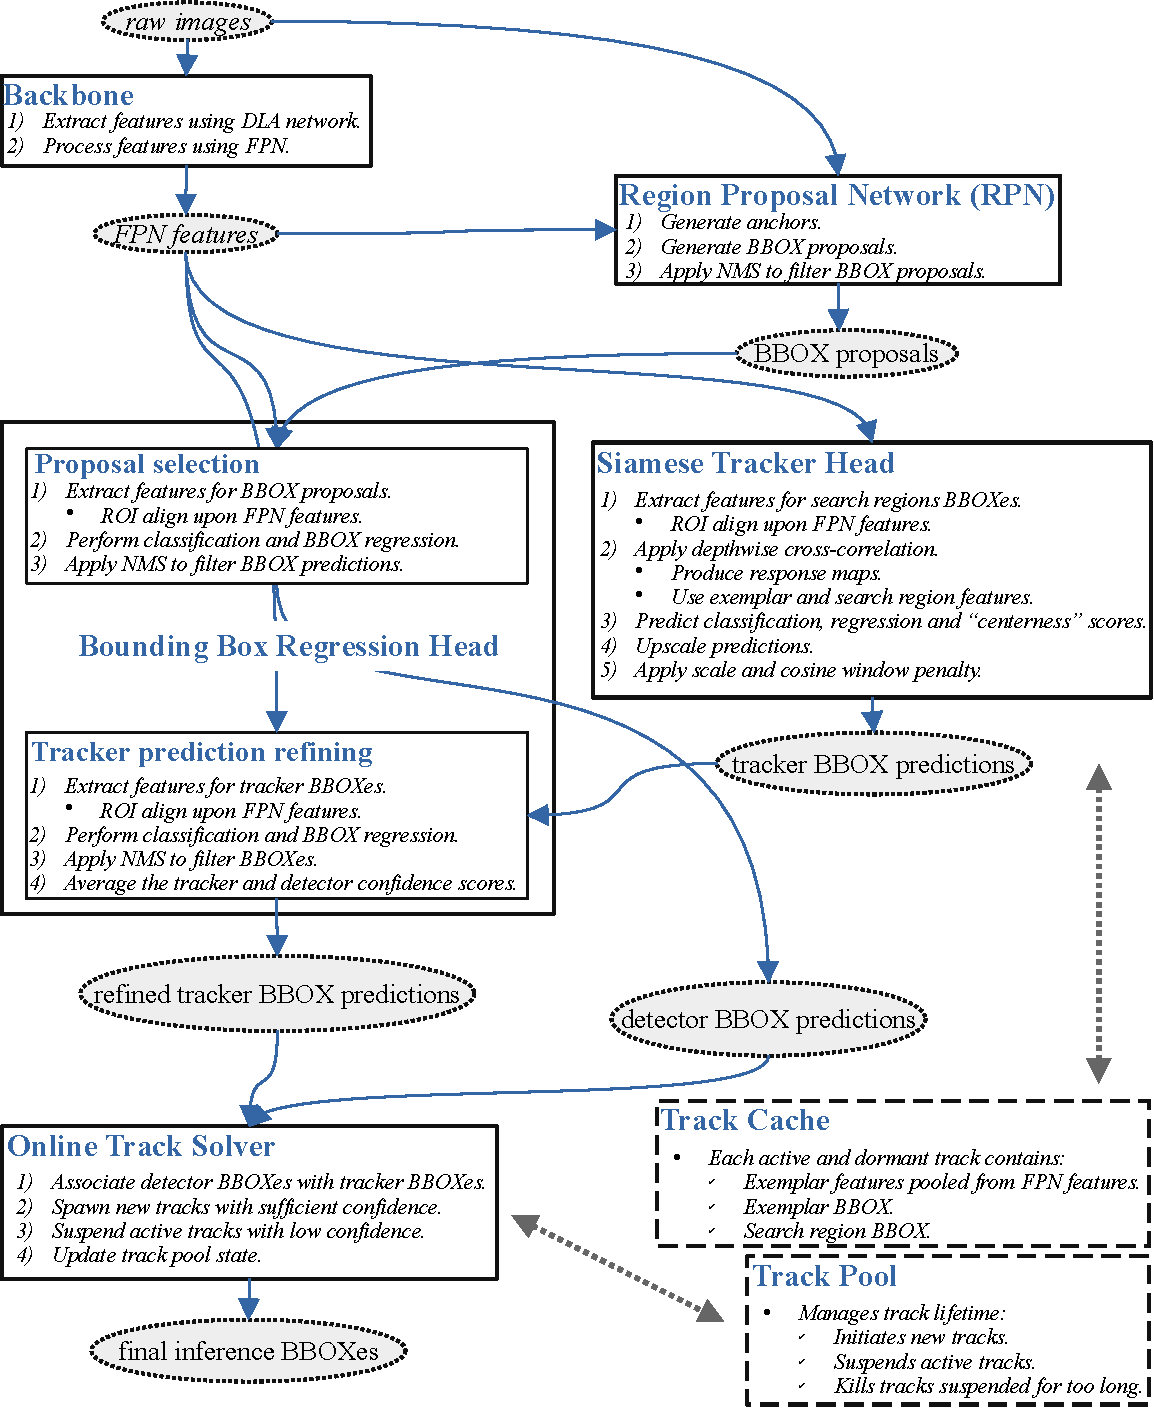
\includegraphics[width=\linewidth]{figures/methodology/siammot_inference_diagram.pdf}
    \caption[\siammot{} inference diagram]{Visualization of the inference pipeline in the \siammot{} architecture. The entire framework efficiently reuses as much information as possible, making it fast and accurate. Backbone features that are a result of intricate \gls{dla} and \gls{fpn} processing are fed into detector and the tracker. Please note that the predictions from the tracker are once again refined using the detector head. Two two aforementioned heads function on top of backbone features through the lens of \gls{roi} align operations. During the inference phase, the ``online solver'' works only with the final \glspl{bbox} produced by the tracker and the object detector. It utilizes a simple caching mechanism to store the backbone features belonging to active or dormant objects. The decision making regarding initialization, suspension and complete removal of track is performed within the ``track pool'' module.}
    \label{fig:SiamMOTInference}
\end{figure}

The spatial-maching is followed by a standard \emph{online} solver that has been widely adopted in numerous works, such as~\cite{bawley2016simple, wojke2017simple, zhou2020tracking, bergmann2019tracking}. In its essence, this solver is simple yet very effective. As our experiments will later demonstrate, it is exceedingly difficult to surpass its performance in general by a significant margin. This solver is governed by the following rules listed below. Let $\subsup{v}{i}{t}$ be the visibility confidence, then
\begin{enumerate}
     \item the object's trajectory is continued as long as its visibility confidence is above a specific threshold $\alpha$, otherwise this trajecotry becomes dormant,
     \item a new trajectory is spawned in case there is a non-matched detection (during the spatial-matching process) and its visibility confidence is above a threshold $\beta$,
     \item a dormant trajectory is terminated, i.e., the object ID will never be used once again, it its visibility confidence is below $\alpha$ for $\tau$ consecutive frames.
\end{enumerate}

\subsubsection{Short-term Occlusion Handling}

This model also attempts to tackle short-term occlusion. It is one of the key incentives that led us to consider this architecture for our experiments, which is the model's ability to handle occlusion in an efficient and trivial manner. At the beginning, we guessed that this phase could be improved upon due to its inherent simplicity. However, regardless of how rudimentary their approach may seem, it implicitly addresses a great deal of frequent cases that apprear in object tracking in a competent way. Our endeavors later described often involved a minor improvement in rare situations with simultaneous minor detriments to common situations. Therefore, the outcome of perfoming worse than the baseline on average was usually inescapable.

A short-term occlusion can be defined as having the visibility confidence for the currently tracker object below the threshold $\alpha$. In \siammot{}, instead of definitely ceaseing the track's existence, the relevant information are kept in memory and thus the search for the exemplar continued until $\tau > 1$ frames have been processed in hope of re-instatiating the object. The most recently predicted location and its corresponding feature frames extracted from the backbone are utilized as the searching template. 

\subsection{Implementation Details}

The \siammot{} model is a paragon of feature pooling.

\subsection{Relevant Implementation-Related Remarks}

In this short section, we would like to summarize several relevant remarks related to the \siammot{} model. 

\subsubsection{Pre-training}

Overall, the model is not difficult to train. By difficult training we mainly mean instability and sensitivity to hyperparameters. However, the training itself requires a great deal of GPU VRAM available in order to use sufficiently large minibatches. As far as our development experience with the \siammot{} model is concerned, we used the \texttt{NVidia}~\cite{webnvidia} \texttt{RTX 2080Ti} graphics cards which provides $4352$ CUDA cores together with $11$GB of GDDR6 memory. For traning, we often exploited an existing backbone model pre-trained on ImageNet~\cite{deng2009imagenet} dataset provided by the authors. Even though there is the entire model available pre-trained on \mscoco{}~\cite{lin2014mscoco} dataset, we decided to avoid it due to conflicting nature of object classes. We observed better performance when training vehicle detection from scratch rather than trying to ``re-wire'' the model to dismiss detecting objects we wanted to avoid in the first place, e.g., pedestrians.

\subsubsection{Gradient Accumulation}

Since majority of our experiments involved expanding the model by adding additional heads, we often struggled with the amount of available GPU VRAM in order to preserve reasonable size of minibatches. To this end, we also experimented with gradient accumulation. This technique allows the user to postpone the model weight updating after more minibatches have been processed. Therefore, the programmer may simulate using larger minibatches than actually are utilized. We emphasize the importance of not updating the model variables must during the accumulation phase so as to to ensure that all the mini-batches are processed by the same model variable values to calculate their gradients. Only after accumulating the gradients of the values of the model weights can be adjusted accordingly.

For a brief illustration, let $w$ be a single weight we want to update with respect to the computed gradient using the loss function $f$. Our goal is to adjust the weight at time $t$ and thus produce the weight at time $t + 1$. The learning rate is denoted by $\alpha$. So, the gradient update is usually performed as
\begin{equation}
    w^{t + 1} = w^t - \alpha \nabla \func{f}{w^t}.
\end{equation}
When using gradient accumulation, the update step is modified as
\begin{equation}
    w^{t + 1} = w^t - \alpha \sum_{i = 1}^{n} \nabla \func{f}{w^t}_i,
\end{equation}
where $n$ is the number of accumulated minibatches.

\begin{figure}[t]
    \centering
    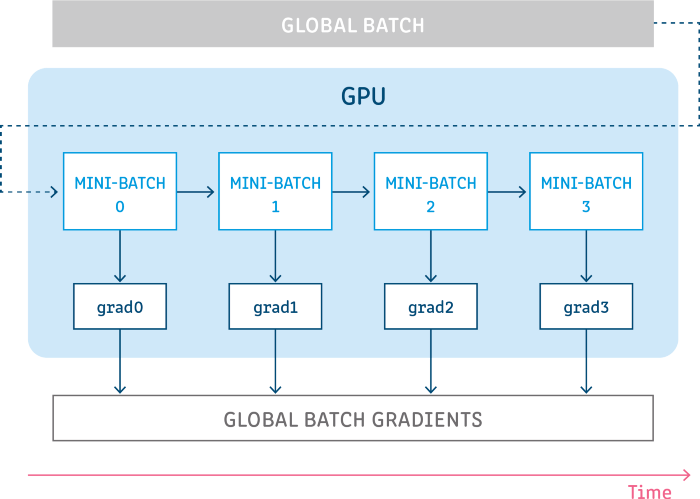
\includegraphics[width=0.7\linewidth]{figures/methodology/gradient_accumulation.png}
    \caption[Gradient accumulation]{Gradient accumulation is a mechanism that allows splitting the minibatch of samples — used for training a neural network — into several even smaller mini-batches of samples that will be processed sequentially. \externalsrc{\cite{webgradaccumulation}}}
    \label{fig:GradientAccumulation}
\end{figure}

Considering the advantages outlined above, it is necessary to acknowledge the potential drawbacks. For example, if batch normalization~\cite{ioffe2015batchnorm} layers are used within the model, then the use of gradient accumulation may possibly have a detrimental effect upon their performance. The reason is that batch normalization layers compute the statistics with respect to a single minibatch. These layers, in their standard formulation and commonly adopted implementation, are incapable of accomodating their innerworkings to adequately administer multiple sequential minibatches. However, there is ongoing research in the direction of group normalization as well, namely works of~\cite{wu2018groupnorm}~and~\cite{zhou2020batchgroupnorm}.

\subsection{Experimental Analysis}